\documentclass[12pt,letterpaper]{article}     % Tipo de documento y otras especificaciones
\usepackage[utf8]{inputenc}                   % Para escribir tildes y eñes
\usepackage[spanish]{babel}                   % Para que los títulos de figuras, tablas y otros estén en español
\addto\captionsspanish{\renewcommand{\tablename}{Tabla}}					% Cambiar nombre a tablas
\addto\captionsspanish{\renewcommand{\listtablename}{Índice de tablas}}		% Cambiar nombre a lista de tablas
\usepackage{geometry}                         
\geometry{left=18mm,right=18mm,top=21mm,bottom=21mm} % Tamaño del área de escritura de la página
\usepackage{ucs}
\usepackage{amsmath}      % Los paquetes ams son desarrollados por la American Mathematical Society
\usepackage{amsfonts}     % y mejoran la escritura de fórmulas y símbolos matemáticos.
\usepackage{amssymb}
\usepackage{graphicx}     % Para insertar gráficas
\usepackage[lofdepth,lotdepth]{subfig}	% Para colocar varias figuras
\usepackage{unitsdef}	  % Para la presentación correcta de unidades
\usepackage{pdfpages}   %incluir paginas de pdf externo, para los anexos
\usepackage{appendix}   %para los anexos
\renewcommand{\unitvaluesep}{\hspace*{4pt}}	% Redimensionamiento del espacio entre magnitud y unidad
\usepackage[colorlinks=true,urlcolor=blue,linkcolor=black,citecolor=black]{hyperref}     % Para insertar hipervínculos y marcadores
\usepackage{float}		% Para ubicar las tablas y figuras justo después del texto
\usepackage{booktabs}	% Para hacer tablas más estilizadas
\usepackage{color}
\batchmode
%\bibliographystyle{plain} 
\pagestyle{plain} 
\pagenumbering{arabic}
\usepackage{lastpage}
\usepackage{fancyhdr}	% Para manejar los encabezados y pies de página
\usepackage{mdframed}
\pagestyle{fancy}		% Contenido de los encabezados y pies de pagina
\setlength{\headheight}{15pt}
\usepackage{multicol}   % Para varias columnas
\usepackage[export]{adjustbox}
\usepackage{ragged2e}
\usepackage{tikz}
\usepackage{pgfplots}
\usepackage{circuitikz}
\usepackage{cancel}
\usepackage{color}
\usepackage{listings}
\usetikzlibrary{shapes.geometric, arrows}
\lstset{ %
language=Rust,                % choose the language of the code
basicstyle=\footnotesize,       % the size of the fonts that are used for the code
numbers=left,                   % where to put the line-numbers
numberstyle=\footnotesize,      % the size of the fonts that are used for the line-numbers
stepnumber=1,                   % the step between two line-numbers. If it is 1 each line will be numbered
numbersep=5pt,                  % how far the line-numbers are from the code
backgroundcolor=\color{white},  % choose the background color. You must add \usepackage{color}
showspaces=false,               % show spaces adding particular underscores
showstringspaces=false,         % underline spaces within strings
showtabs=false,                 % show tabs within strings adding particular underscores
frame=single,           % adds a frame around the code
tabsize=2,          % sets default tabsize to 2 spaces
captionpos=b,           % sets the caption-position to bottom
breaklines=true,        % sets automatic line breaking
breakatwhitespace=false,    % sets if automatic breaks should only happen at whitespace
escapeinside={\%*}{*)}          % if you want to add a comment within your code
}
\tikzstyle{startstop} = [rectangle, rounded corners, minimum width=3cm, minimum height=1cm,text centered, draw=black, fill=red!30]
\tikzstyle{thread} = [trapezium left angle=70, trapezium right angle=110, minimum width=3cm, minimum height=1cm, text centered, draw=black, fill=green!30]
\tikzstyle{process} = [rectangle, minimum width=3cm, minimum height=1cm, text centered, text width=3cm, draw=black, fill=orange!30]
\tikzstyle{decision} = [diamond, text centered, draw=black, fill=blue!30]
\tikzstyle{arrow} = [thick,->,>=stealth]
%%%%
%---------------------------Definición del environment resumen---------------------------
\newcounter{resumen}
\setcounter{resumen}{0}
\def\theejemplo{\thechapter.\arabic{resumen}}

\newenvironment{resumen}
{	
	\begin{center}
	\begin{minipage}[t]{500 pt}
	\vspace{5mm}
	\emph{\textbf{Resumen}}
	\\[-2mm]
	\line(1,0){500}
	\\[-4.25 mm]
	\line(1,0){500}
	\vspace{\baselineskip}
}
{
	\normalsize
	\\[2mm]
	\footnotesize\textbf{Palabras clave: \footnotesize\@palabras}
	\\[-2mm]
	\line(1,0){500}
	\\[0.5cm]
	\end{minipage}
	\end{center}
}

% -------------------- Para las palabras clave -------------- %
\def\palabras#1{\gdef\@palabras{#1}}

%---------------------------Definición del float circuito---------------------------
\newfloat{circuito}{thp}{lop}
\floatname{circuito}{Circuito}

%---------------------------Definición del float código---------------------------
\newfloat{codigo}{thp}{lop}
\floatname{codigo}{Código}

%%%%%%%%%%%%%%%%%%%%%%%%%%%%%%%%%%%%

\lhead{B5692 - Plataforma de programación y prueba para PCB}
\chead{}
\rhead{Desarrollo de maqueta y HMI}	% Aquí va el numero de experimento, al igual que en el titulo
\lfoot{Ingeniería Electrónica}
\cfoot{\thepage\ de \pageref{LastPage}}
\rfoot{Universidad Nacional de Río Negro}

%%%%%%%%%%%%%%%%% PALABRAS CLAVE 
\palabras{Punto de trabajo, pequeña señal, analíticamente, simulación, laboratorio}
%%%%%%%%%%%%%%%%%
% Se escriben después del resumen y sintetizan los conceptos fundamentales del experimento a modo de etiquetas


%%%%%%%%%%%%%%%%
\begin{document}	% Inicio del documento
%%%%%%%%%%%%%%%%
\pdfbookmark[1]{Portada}{portada} 	% Marcador para el título

\begin{titlepage}
\centering
{
\includegraphics[width=0.2\textwidth]{imagenes/LOGOUNRN.jpg}\par}
\vspace{0.5cm}
{\bfseries\large Universidad Nacional de Río Negro \par}
\vspace{0.5cm}
{\scshape\large Escuela de Producción, Tecnología y Medio Ambiente \par}
\vspace{0.5cm}
{\scshape\large Ingeniería Electrónica \par}
\vspace{3cm}
{\bfseries\Large Plataforma de programación y prueba para PCB \par}
{\Large Desarrollo de maqueta y HMI\par}
\vfill
{\large \textbf{Alumno:} Mirko Manuel Pojmaevich\par}
{\large \textbf{Profesores:} Gelardi Gustavo\par}
{\large \textbf{Materia:} Electrónica Analógica | \textbf{Código:} B5692\par}
\vspace{3cm}
{\large Fecha de entrega: 10 de noviembre de 2022 \par}
\vspace{1cm}
\begin{table*}[!ht]
\begin{center}
\begin{tabular}{| c | c | c | c |}
\hline
\textbf{Rev.} & \textbf{Fecha} & \textbf{Profesor} & \textbf{Nota} \\ 
\hline
 &  & & \\
 \hline
 & & &  \\
\hline
\end{tabular}
\end{center}
\end{table*}
\end{titlepage}
%\maketitle							% Título
\newpage
\tableofcontents
\newpage
\listoffigures
%\listoftables

\newpage
%palabras claves
\section{Resumen}
%%%%%%%%%%%%%%%%%%%
\begin{resumen}
	Se presenta un sistema automático para la validación de circuitos electrónicos.
	Este inyecta señales en la placa siendo probada y mide las respuestas.
	Es capaz de medir tanto señales digitales como niveles analógicos de tensión.
	Para circuitos que incluyen un microcontrolador, de tipo PIC, el sistema es capaz de programar
	firmware, permitiendo probar la correcta funcionalidad de los módulos internos
	del dispositivo. El sistema clasifica los circuitos probados separando los
	funcionales de los defectuosos de acuerdo al conjunto de reglas que se le den.
	El estado de las pruebas puede ser monitoreado mediante un HMI.
\end{resumen} 
%%%%%%%%%%%%%%%%%%% 
%\section{Objetivos} 
% 
%\begin{itemize} 
%\item Aplicar mediante un ejemplo práctico conocimientos vistos en la materia.
%\item Ampliar conocimientos y herramientas referidas a filtros.
%\end{itemize}
%\newpage
%%%%%%%%%%%%%%%%%%%%%%%%%%%%%%%%%%
\section{Marco teórico}
\label{Marco teórico}

\subsection{Pogopins}

Se conoce como Pogopin a un tipo de contacto con muelle como el que se muestra en la figura \ref{fig:pogopin}.
Este permite realizar una conexión con una circuito impreso con únicamente un pad expuesto de forma robotizada.

\begin{figure}[!ht]
\centering
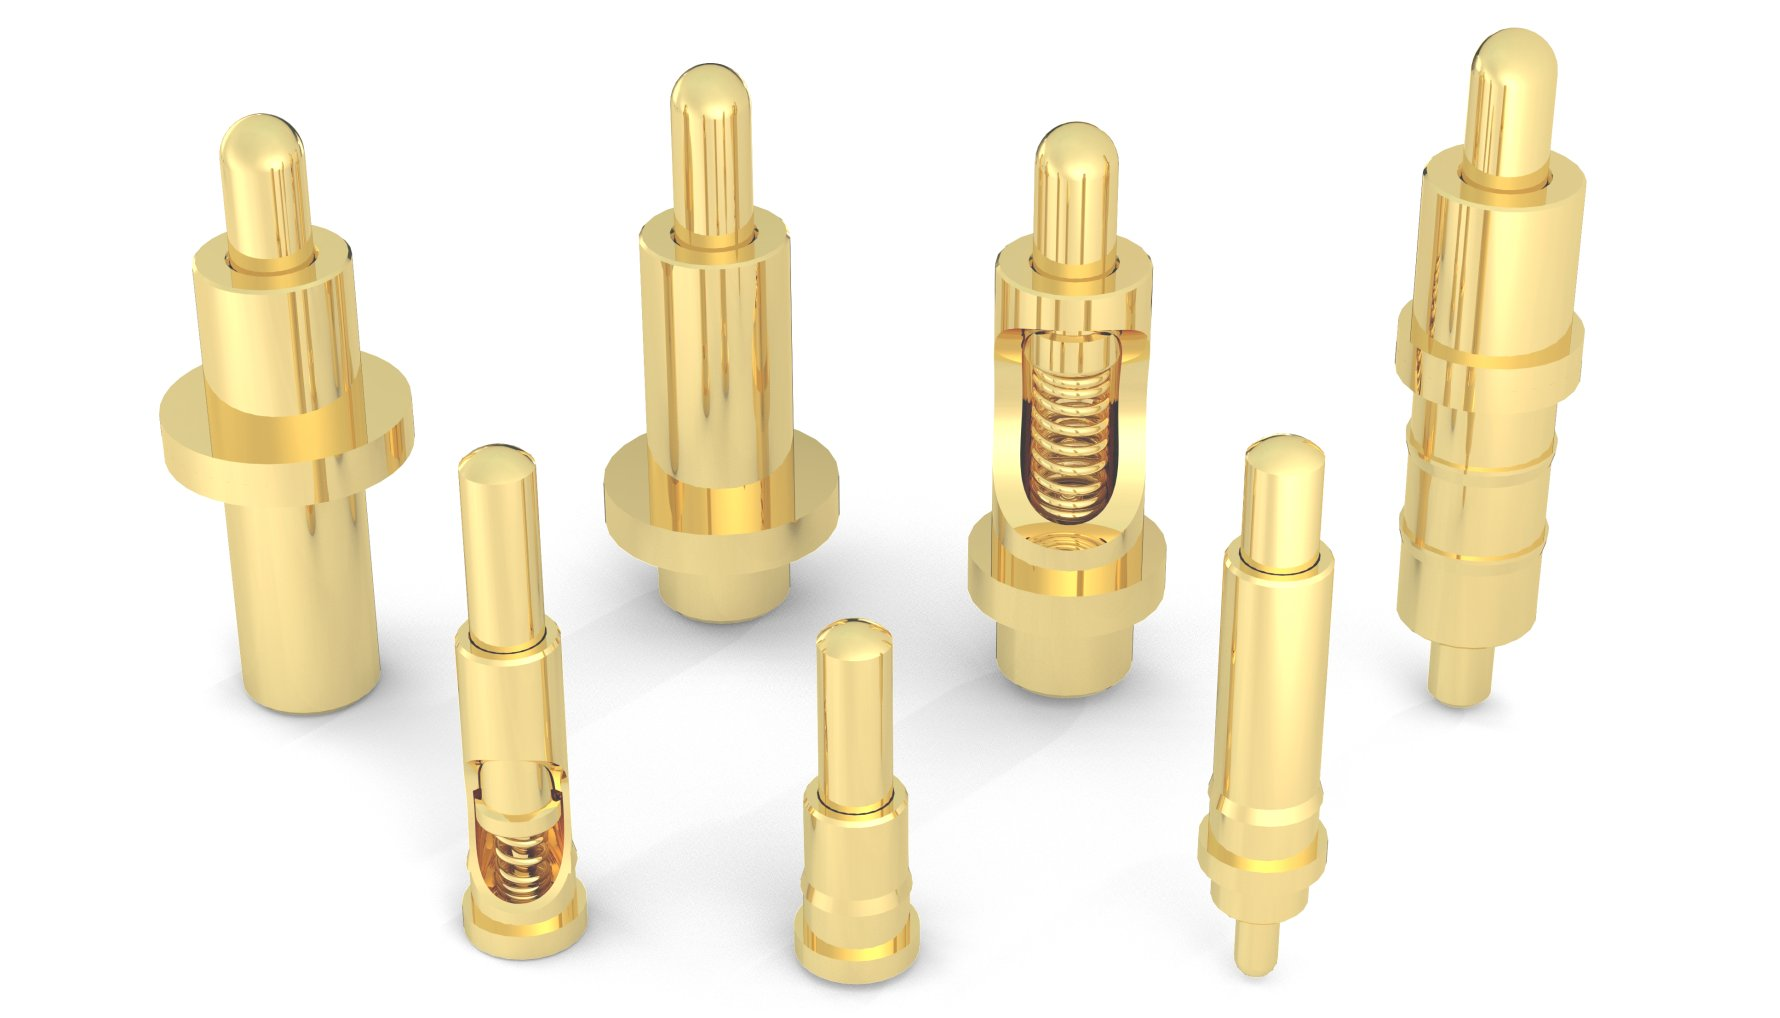
\includegraphics[]{imagenes/pogopin.jpg}
\caption{Ejemplo de Pogopins}
\label{fig:pogopin}
\end{figure}

\subsection{SBC}

SCB son las siglas en ingles de Single Board Computer, refieren a una computadora completamente contenida en una
única placa de circuito impreso. El ejemplo mas popular es la RaspberryPi.

\subsection{/dev}

En el sistema de directorios de Linux el directorio \textbf{/dev} es uno que contiene archivos especiales 
o de tipo dispositivo. En su mayoría los archivos contenidos en este directorio permiten interactuar con el
hardware, tratando a los dispositivos físicos del sistema como parte del sistema de ficheros. Esto funciona 
asociando los canales de lectura y escritura de los archivos con los dispositivos físicos. Por ejemplo,
si se escribe al archivo \textbf{/dev/dsp}, el cual representa los parlantes, se escuchará un sonido. Para el correcto
funcionamiento de los dispositivos se debe respetar el protocolo mediante el cual se interactúa con estos archivos.

\subsubsection{Módulos del kernel}

No todos los archivos bajo \textbf{/dev} representan un dispositivo, algunos representan extensiones del kernel de Linux.
Estas extensiones generalmente interactúan con uno o mas dispositivos físicos bajo un protocolo distinto, esto
con el fin de encapsular, simplificar o incluso hacer posibles ciertas funcionalidades. Por ejemplo,
existe una extensión de kernel para el manejo de LCDs, estos podrían ser controlados mediante escritura a los
ficheros de entrada-salida o algún fichero de un módulo de comunicación serie, en ambos casos lo que se 
escribe en los archivos de \textbf{/dev} no es lo que se desea obtener, sino que se debe traducir el mensaje mediante el
software y realizar múltiples llamados al sistema desde el entorno de usuario para la escritura. En el caso de un
módulo de kernel dedicado, se puede escribir la información final que se desea obtener, la traducción y envío del
mensaje ocurrirá en espacio del kernel de forma muy eficiente con una única llamada al sistema. 

\subsection{Rust}

Es un lenguaje de programación de sistemas orientado a la seguridad y la eficiencia. 
Rust es un lenguaje compilado de alto nivel, que no utiliza un recolector de basura, 
como lo hace Java por ejemplo. Permite un control fino de la memoria similar al de 
C o C++, pero a diferencia de estos, Rust no utiliza un paradigma de alocación y 
liberación explicita de memoria, sino que se basa un ``Borrow checker''.
El ``Borrow checker'' consiste de un conjunto de reglas que limitan como se puede 
programar en Rust, respetando estas reglas se obtienen un conjunto de garantías.
Estas garantías incluyen un código libre de fugaz de memoria, inmunidad a condiciones 
de carrera y validez de los datos al los que se accede. 
Existen situaciones en las que el ``Borrow checker'' es demasiado estricto y para
garantizar la seguridad opta por no compilar un código valido, antes que dar por valido
un programa que pudiera fallar en algún escenario. Esto puede ser un problema cuando 
se tiene un que acceder al hardware, por ejemplo si se quiere acceder a algún registro 
de la plataforma que se esta utilizando, el ``Borrow checker'' no tiene forma de garantizar
que dicho registro exista, depende del programador conocer la plataforma en la que se va a 
ejecutar el programa, para ello existe un tipo de bloque de código llamado ``unsafe'', todo
programa contenido en un bloque con esta etiqueta será compilado sin revisión del ``Borrow checker''.

\clearpage
\section{Materiales}

En esta sección se describen los elementos utilizados para la realización del proyecto, no se discute si la
elección fue óptima porque estos son productos de los que se disponía con antelación.

\subsection{NanoPi Neo3}

El NanoPi Neo3 es una SBC compacta y de bajo costo. Utiliza un CPU Rockchip RK3328 de cuatro núcleos, con
arquitectura ARM Cortex-A53. Cuenta con 1 ó 2 GB de memoria RAM, y Gbps Ethernet. 

\begin{figure}[!ht]
\centering
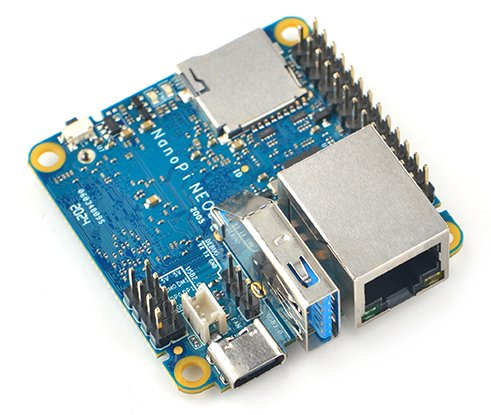
\includegraphics[scale=0.5]{imagenes/naopi.jpg}
\caption{NanoPi Neo3}
\label{fig:nanopi}
\end{figure}

Esta SCB interactúa con los sensores y motores coordinando el funcionamiento de la plataforma.
A su vez, esta se encarga de programar los microcontroladores, inyectar las señales y leer 
las respuestas digitales. Como la mayoría de SCBs no contienen un ADCs incorporado, se utiliza
un dispositivo externo para la medición analógica de niveles de tensión, los que luego son
comunicados mediante el protocolo I2C.

Por último, este SCB actúa como host de un servidor TCP, para que múltiples usuarios puedan acceder
al HMI de forma remota.

\subsection{PIC18F45K50}

Este microcontrolador es el dispositivo externo antes mencionado, que actúa como ADC y comunica los
valores de tensión medidos mediante I2C. Este resulta mucho mas capaz de lo requerido para la tarea.

\subsection{Motorreductor}

Para movilizar la cinta se utiliza un motor con una reducción 1:48 y salida en doble eje TT de marca
genérica similar al que se muestra en la figura \ref{fig:motor}.

\begin{figure}[!ht]
\centering
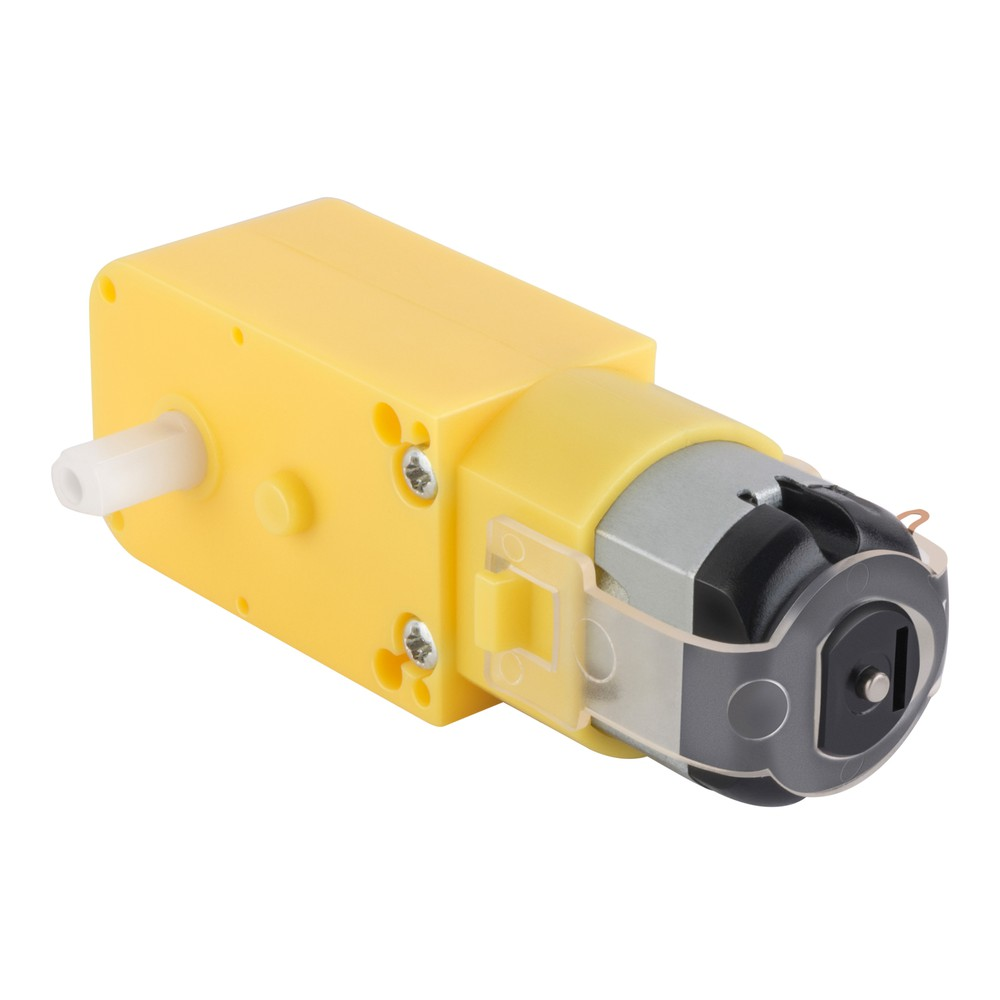
\includegraphics[scale=0.25]{imagenes/motorreductor.jpg}
\caption{Motorreductor}
\label{fig:motor}
\end{figure}

\subsection{Servo motor}

Los servo motores utilizados son micro servos, modelo MG90S, de la marca Tower Pro, como el que
se muestra en la figura \ref{fig:servo}. Este cuenta con un torque de $1,8\kilogram f$ a $4,8\volt$
y $2,2\kilogram f$ a $6\volt$.

\begin{figure}[!ht]
\centering
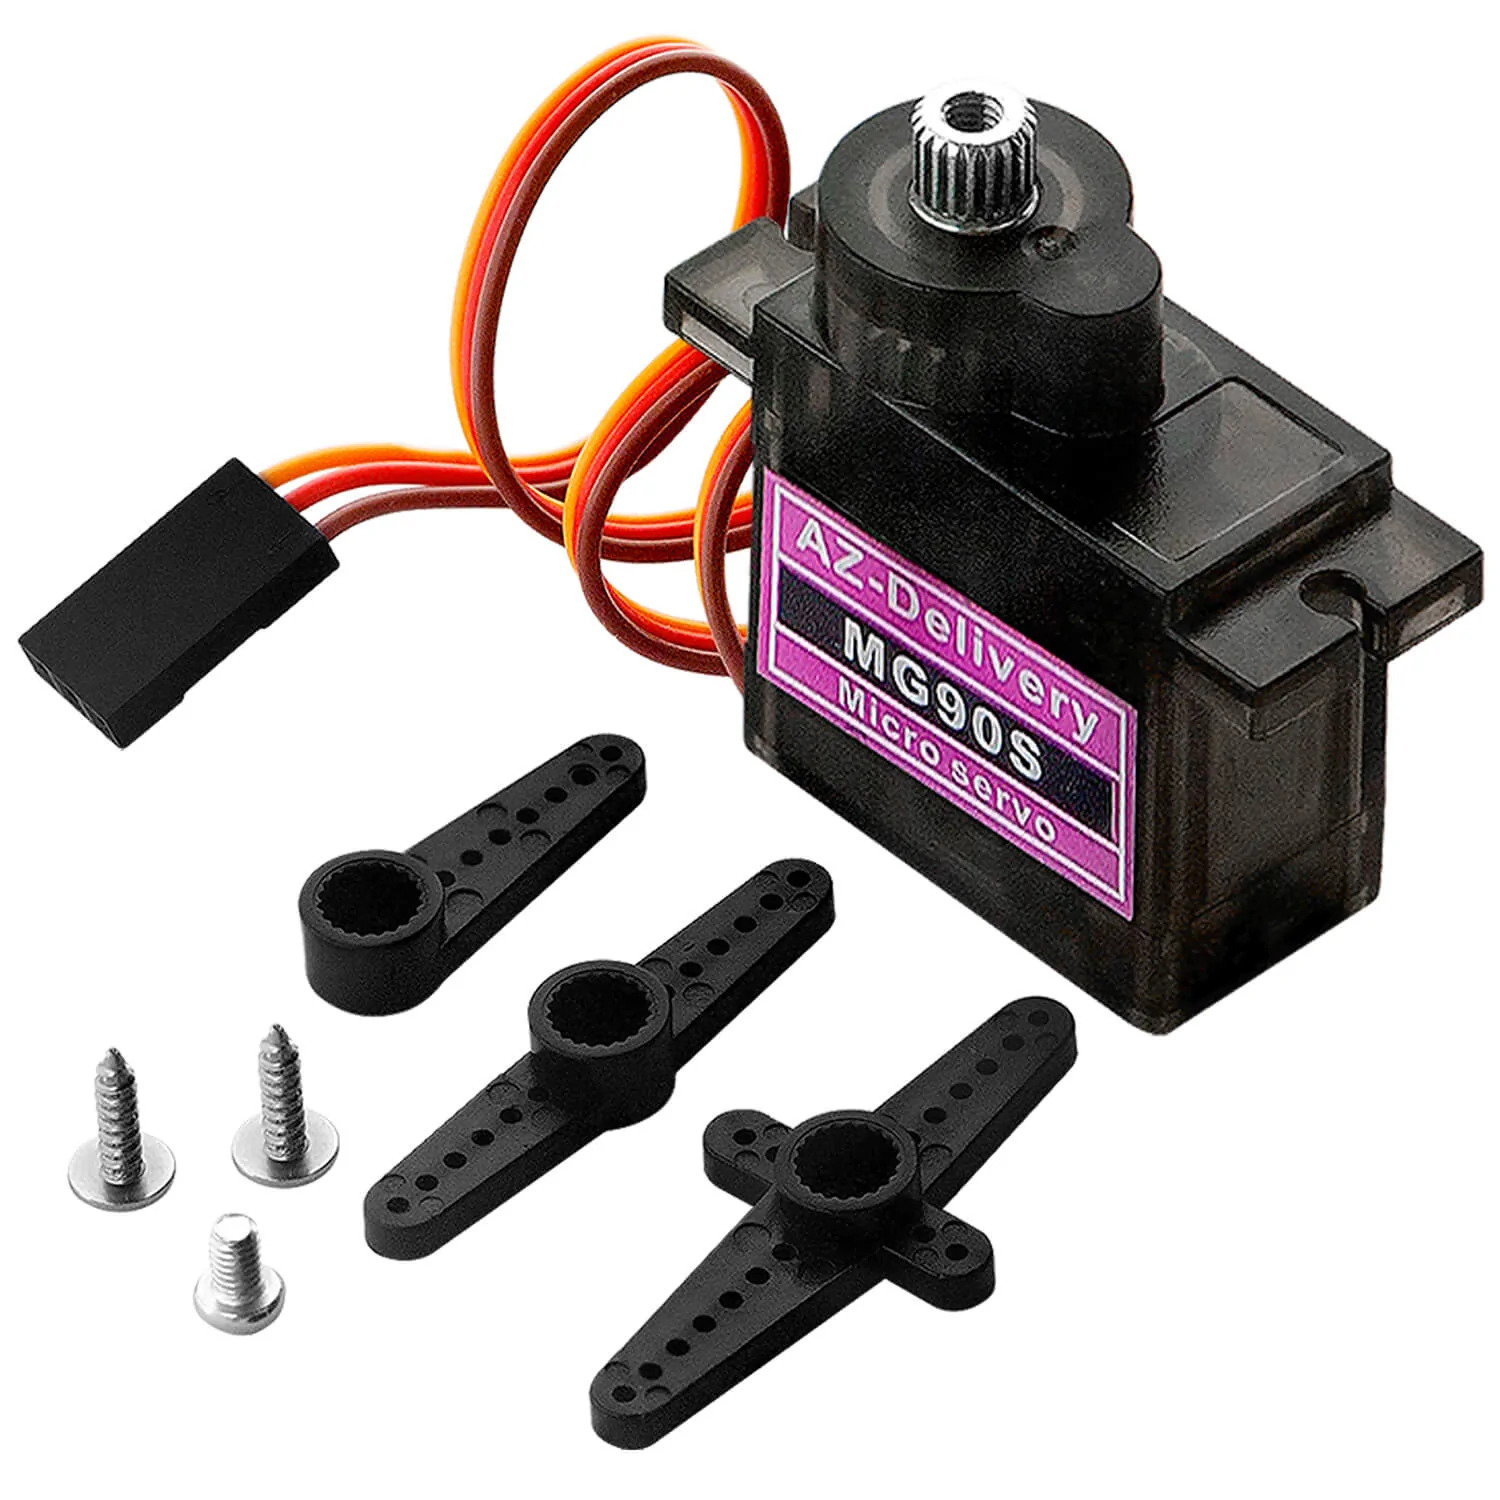
\includegraphics[scale=0.15]{imagenes/servo.jpg}
\caption{Servo motor}
\label{fig:servo}
\end{figure}

\subsection{Sensor óptico}

Para detectar la presencia de una placa en los puntos relevantes del proceso, se utilizaron sensores ópticos.
Estos consisten en un led y un fototransistor, dispuestos de manera tal que el led permita que el fototransistor
sature, la detección ocurre cuando un objeto obstruye el paso de luz, causando que el fototransistor entre en
corte. Su aspecto y diagrama esquemático se pueden ver en la figura \ref{fig:sensoptico}.

\begin{figure}[!h]
	\begin{minipage}{.5\textwidth}
		\begin{center}
			\begin{circuitikz}[american,]
				\draw (0,0) node[npn, photo](Q1){};
				\draw (Q1.E) to[short]
					++(0,0)
					to[short]
					++(-2,0)
					node[](gnd){};
				\draw (Q1.C) to [short, -o] 
					++(1.5, 0)
					node[](out){};
				\draw (-2,0.6) 
					to[leD]
					++(0,-1)
					to[short]
					(gnd |- gnd);
				\draw (-2,0.6)
					to[short]
					(gnd |- out)
					to[short, -o]
					++(-1.5,0);
				\draw (-1,-0.77)
					to[short, *-o]
					++(0,-1);
			\end{circuitikz}
		\end{center}
	\end{minipage}%
	\begin{minipage}{.5\textwidth}
		\begin{center}
			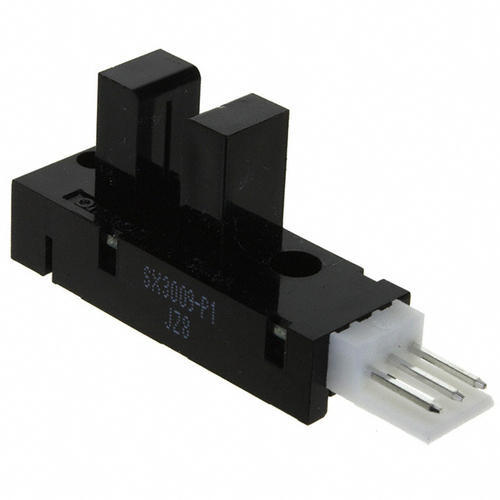
\includegraphics[scale=0.3]{imagenes/optico.jpg}
		\end{center}
	\end{minipage}
\caption{Sensor óptico}
\label{fig:sensoptico}
\end{figure}

\section{Estructura}

Para automatizar las pruebas sobre los circuitos se suele utilizar una cama de Pogopins, 
estas pueden estar completamente robotizadas, como la que se presenta, o pueden ser manuales,
como la que se muestra en la figura \ref{fig:pogojig}.

Para la construcción de esta plataforma se decidió un diseño basado en una cinta transportadora.
Esta llevaría las placas hasta que estén debajo de la cama de pines, donde un sensor óptico detectaría 
su presencia, deteniendo la cinta. Con la placa bajo la cama, un servo motor conectado a una leva 
bajaría la cama. Con los Pogopins haciendo contacto con la placa, se quemaría el firmware de prueba.
Luego se inyectarían señales de acuerdo a una rutina de prueba y se medirán respuestas tanto digitales
como analógicas. En base a las respuestas se clasifica la placa como valida o defectuosa. Dependiendo 
de la clasificación dada se posicionaría, mediante un servo motor, un selector de dirección. Por último
la cinta volvería a encenderse. Para evitar que la cinta se detenga, por una placa nueva para probar,
antes de que la placa ya probada llegue al selector; se utilizan utilizan dos cintas independientes, 
con un sensor óptico cerca del final de cada una. La primera se detiene cuando una placa llega a la
posición de prueba, y la segunda cuando una la ultima placa pasa el selector.

\begin{figure}[!ht]
\centering
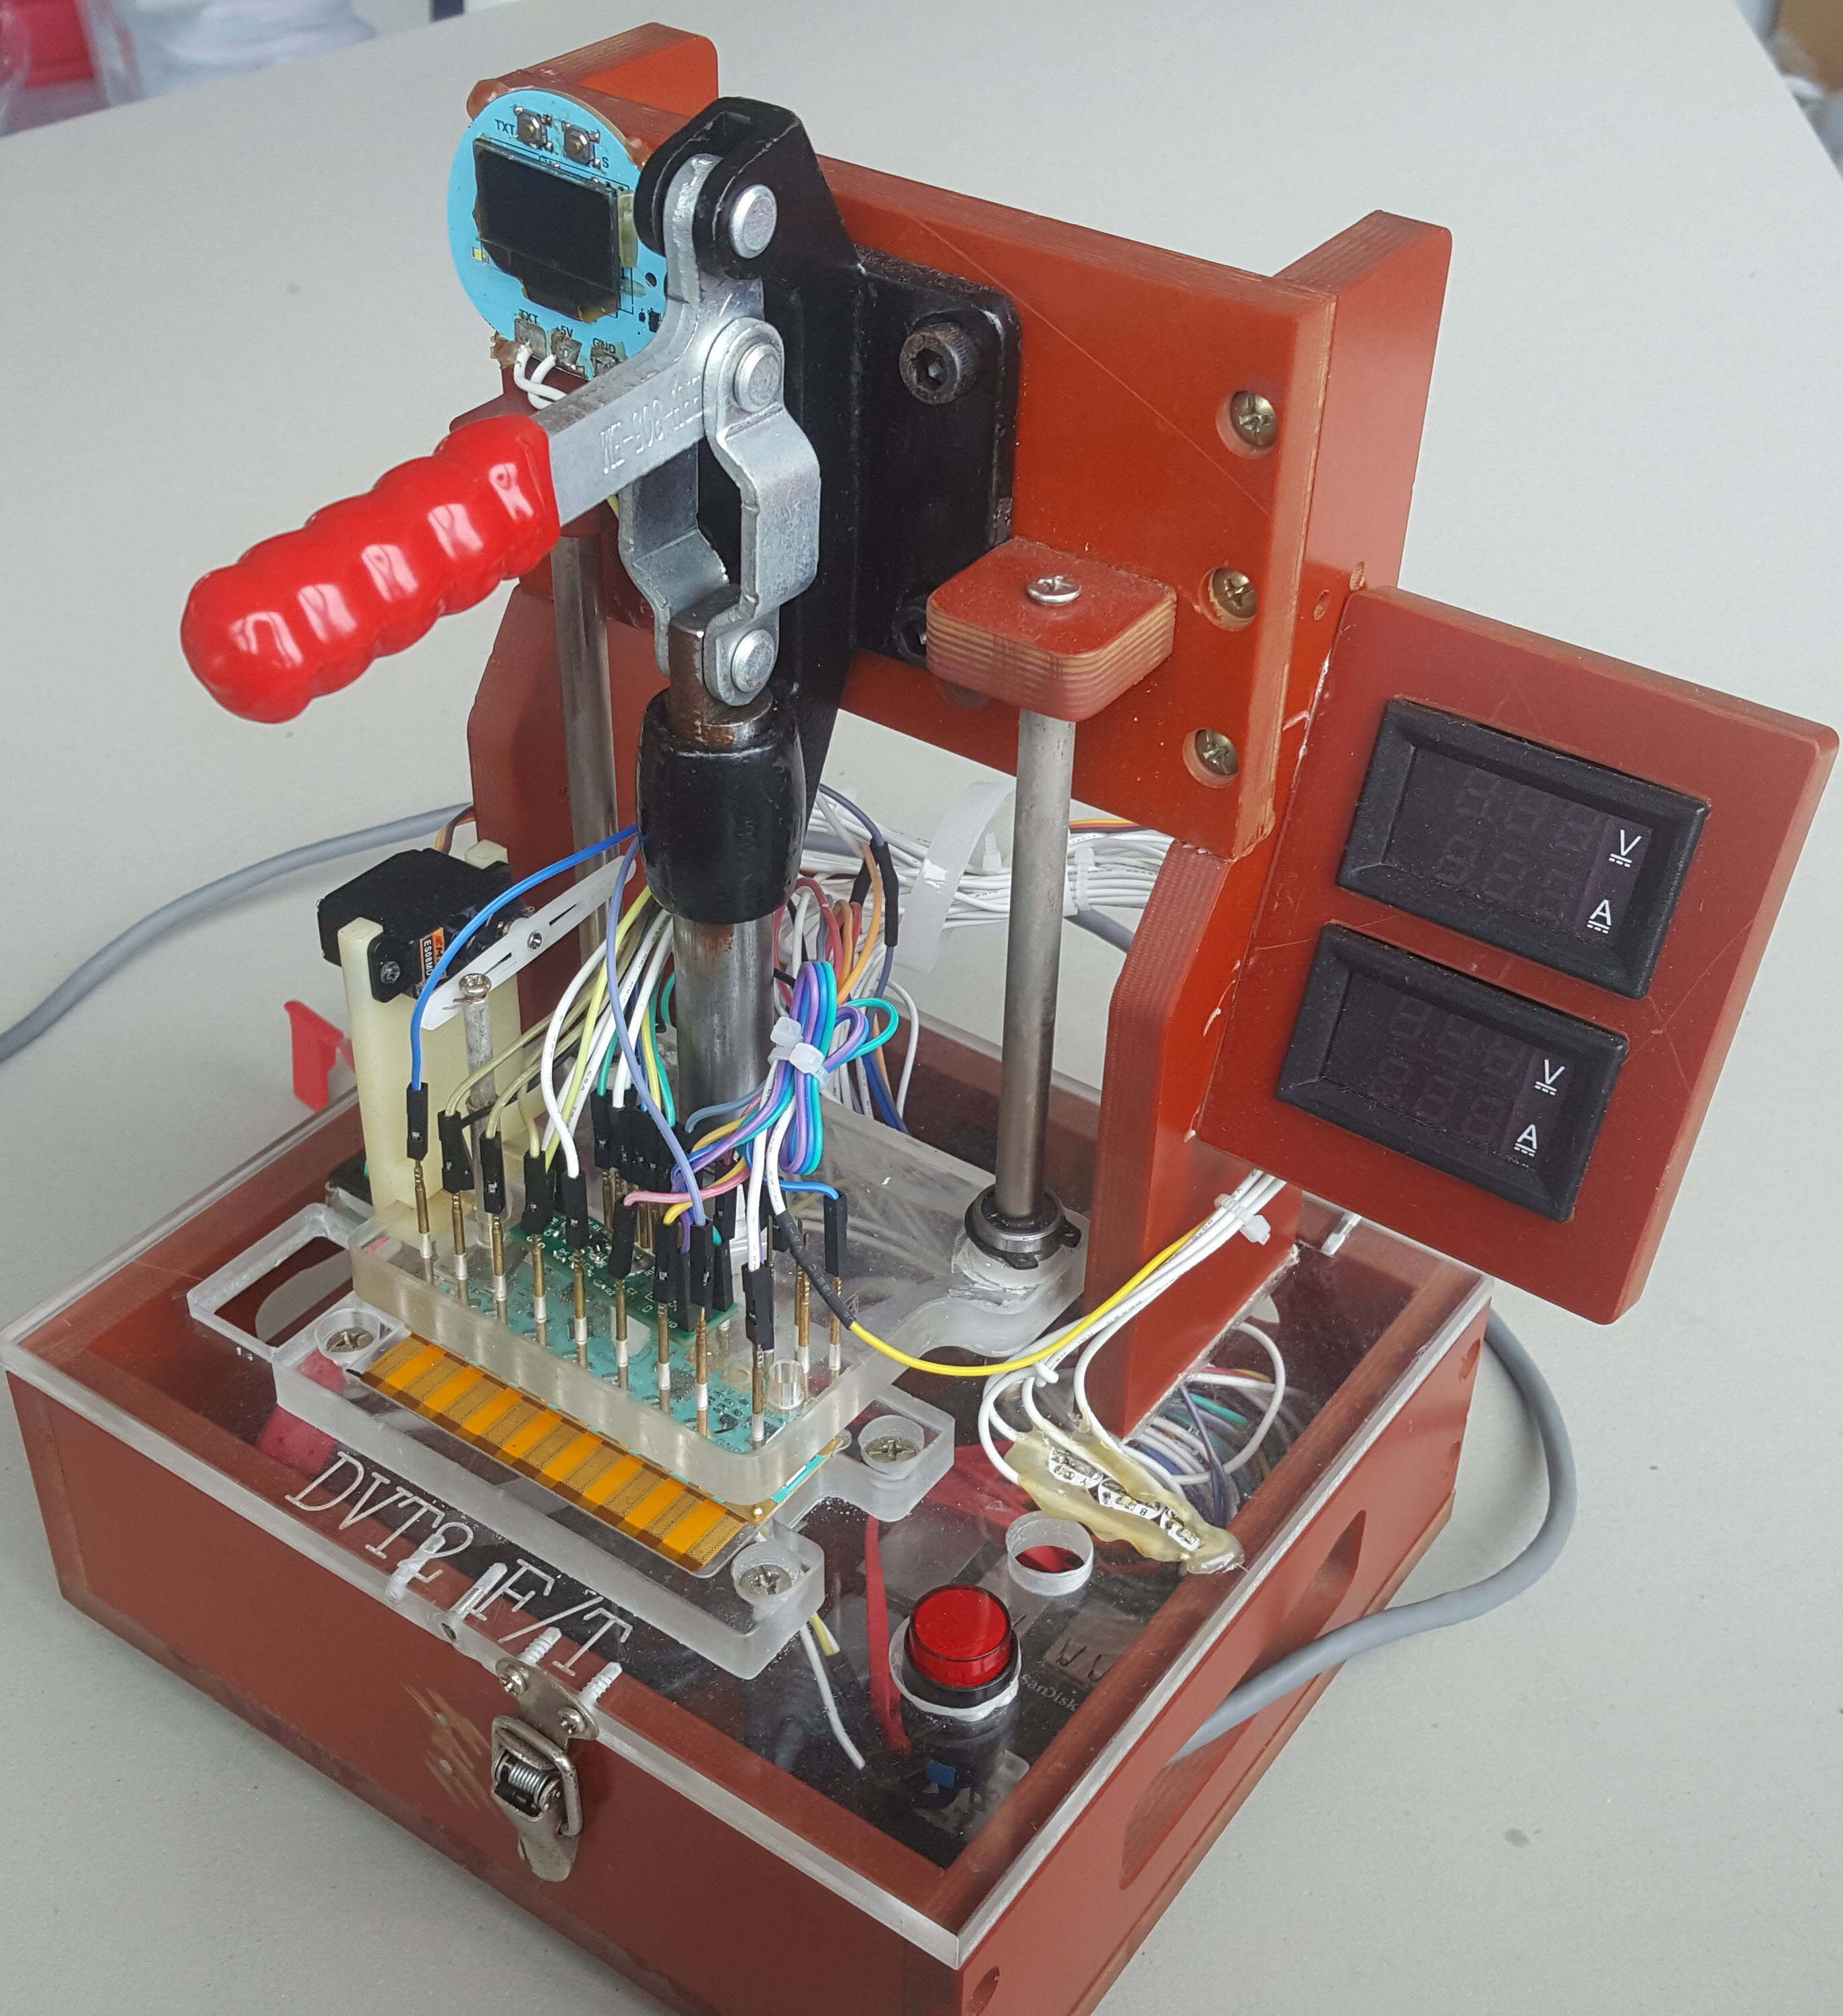
\includegraphics[scale=0.1]{imagenes/pogojig.jpg}
\caption{Ejemplo de ``test jig manual''}
\label{fig:pogojig}
\end{figure}

\section{Pickle}

Para poder realizar la programación de los PIC se utiliza el software Pickle. 
Este provee un mecanismo para interactuar con el microcontrolador y quemar en él un firmware.
Su instalación es sencilla y puede lograrse con los comandos mostrados en el Código \ref{code:instalacionPickle}.
Sin embargo, este sólo posee soporte nativo para una contada selección de SBCs populares. En el caso del NanoPi NEO3,
el programa depende de un módulo externo del kernel de Linux llamado GPIO BIT BANG.
Compilar módulos del kernel requiere de la instalación de los headers del kernel, los cuales están asociados al kernel
que se tiene instalado, el que a su vez depende de la arquitectura en la que se trabaje. Los paquetes de headers en los
repositorios de Linux suelen seguir un consenso en sus nombres, bajo la siguiente estructura, 
\textit{linux-headers-\$(uname -r)}. En el caso del NanoPi NEO3, este consenso se rompe siendo el nombre del paquete, 
\textit{linux-headers-current-rockchip64}. Una vez instalados los headers del kernel, uno debe asegurarse de que exista
un enlace simbólico, del directorio \textbf{/lib/modules/\$(uname -r)/build} al directorio \textbf{/usr/src/}.
Una vez que todas las herramientas para la extensión del kernel estén en su lugar, se puede instalar el módulo 
GPIO BIT BANG mediante los comandos mostrados en el Código \ref{code:instalacionGPIOBB} (el comando \textit{hg} requiere
de la instalación de mercurial).

\begin{codigo}[]
	\begin{lstlisting}
	cd /tmp
	wget http://wiki.kewl.org/downloads/pickle-4.20.tgz 
	tar zxf pickle-4.20.tgz 
	cd pickle-4.20/
	make
	sudo make install
	\end{lstlisting}
	\caption{Instalación Pickle}
	\label{code:instalacionPickle}
\end{codigo}

\begin{codigo}[!h]
	\begin{lstlisting}
	hg clone http://hg.kewl.org/pub/gpio-bb
	cd gpio-bb
	make
	sudo make install
	\end{lstlisting}
	\caption{Instalación GPIO BIT BANG}
	\label{code:instalacionGPIOBB}
\end{codigo}

Pickle se configura por medio de un archivos llamado .pickle donde se especifica que mecanismo se va a utilizar 
para programación, así como a que pines está conectada cada linea de programación del ICSP. En el código 
\ref{code:.pickle} se puede ver un ejemplo de una configuración para GPIO BIT BANG.
Los números asignados a cada linea indican el número de pin para Linux, el cual varia en cada dispositivo pero
suele estar bien documentado. En el caso del NanoPi Neo3, los gpio estan distribuidos en 5 grupos, estos figuran 
bajo \textbf{/dev}, como \textbf{gpiochipo0}, \textbf{gpiochipo1}, \textbf{gpiochipo2}, \textbf{gpiochipo3} y
\textbf{gpiochipo4}. Dento de cada grupo hay 32 pines, numerados del 0 al 31. El número de pin de Linux es único,
y se calcula como $(N^\circ\ de\ gpiochip)\cdot32\ +\ (N^\circ\ interno\ en\ el\ chip)$. Por ejemplo, el pin número
cuatro, del gpiochip2, lleva el número $2\cdot32+4=68$ para Linux.

\begin{codigo}[!h]
	\begin{lstlisting}
	PURA MIERDA CAMBIAR ESTO
	\end{lstlisting}
	\caption{Ejemplo de configuración de Pickle para GPIO BIT BANG}
	\label{code:.pickle}
\end{codigo}

\section{Cinta}

Para controlar la cinta se implementó un programa en Rust, que controla la cinta prendiendo y apagando un motor
en función de eventos, como flancos ascendentes y descendentes en el pin conectado a un sensor óptico.
La conexión con el sensor se muestra en el circuito \ref{cir:sensor-pin}.
El principio de funcionamiento para las primera cinta es muy simple, prender el motor y mantenerlo así hasta
ver un flanco ascendente en el pin del sensor, luego dar la orden de iniciar las pruebas, una vez terminadas las
pruebas repetir el proceso. Este concepto tiene el problema de que la velocidad de transición del sensor óptico
es muy lenta. Lo que causa que se detecten muchos flancos cada vez que una placa llega. La programación utilizada
es orientada a eventos, no a interrupciones, por lo que cada evento de flanco es agregado a una cola FIFO y leída
cuando se consulta. Esto causa que si una placa al llegar genera diez eventos, la rutina de parar la cinta, bajar
la cama e intentar realizar las pruebas, se ejecutará diez veces a pesar de que hubiera una única placa. 
Esto se solucionó midiendo el sensor en cada evento, e ignorando los eventos donde no había placa, esta solución
se muestra en el código \ref{code:cinta1}, aquí el testeo de la placa se representó como una espera de cinco segundos.
La solución fue efectiva cuando se estaba utilizando un led para simular el motor, una vez puesto el motor,
como se muestra en el circuito \ref{cir:motor-pin}, que
se planeaba utilizar, este inyectó pulsos inesperados, que fueron erróneamente detectados como eventos, y estos 
podían ocurrir aun con una placa en el sensor, lo que causa que el evento no se descarte. Este nuevo problema
se solucionó con un capacitor paralelo al motor.
Por ultimo, para poder integrar este principio en el resto del proceso es necesario enviar un mensaje al segundo
tramo de cinta dando aviso de que una placa acaba de ser probada.

\begin{circuito}[!h]
	\begin{center}
		\begin{circuitikz}[american,]
			\draw (0,0) node[npn, photo](Q1){};
			\draw (Q1.E) to[short]
				++(0,0)
				to[short]
				++(-2,0)
				node[](gnd){};
			\draw (Q1.C) to [short, *-o] 
				++(1.5, 0)
				node[right](out){$GPIO$};
			\draw (Q1.C) to [R=$10\kiloohm$] 
				++(0,2)
				node[vcc](vcc){$3\volt 3$};
			\draw (-2,0.6) 
				to[leD]
				++(0,-1)
				to[short]
				(gnd |- gnd);
			\draw (-2,0.6)
				to[R=$330\ohm$]
				(gnd |- vcc)
				node[vcc](){$3\volt 3$};
			\draw (-1,-0.77)
				to[short, *-]
				++(0,-1)
				node[ground](){};
		\end{circuitikz}
	\end{center}
\caption{Conexión del sensor óptico al NanoPi Neo3}
\label{cir:sensor-pin}
\end{circuito}

\begin{codigo}[!h]
	\begin{lstlisting}
	PURA MIERDA CAMBIAR ESTO
	\end{lstlisting}
	\caption{Código para controlar el primer tramo de cinta}
	\label{code:cinta1}
\end{codigo}

\begin{circuito}[!h]
	\begin{center}
		\begin{circuitikz}[american,]
			\draw (0,0) node[nigfete,solderdot](Q1){};
			\draw (0,1.5) node[elmech](motor){M};
			\draw (Q1.S) to[short]
				++(0,0)
				node[ground](gnd){};
				\draw (Q1.D) 
					to[short] 
					(motor.bottom);
				\draw (motor.north) 
					to[short]
					++(0,0)
					node[vcc](){5\volt};
				\draw (Q1.G)
					to[R=$10\kiloohm$]
					++(-2,0)
					to[short, -o]
					++(-0.1,0)
					node[left](){$GPIO$};
		\end{circuitikz}
	\end{center}
\caption{Conexión del motorreductor al NanoPi Neo3}
\label{cir:motor-pin}
\end{circuito}

La lógica del segundo tramo es aun más simple, esperando en un bucle el mensaje
de que una placa fue probada, y ante su
llegada encendiendo la cinta hasta el evento de que la placa pasó el selector.
Esta implementación se muestra en el código \ref{code:cinta2}.

\begin{codigo}[!h]
	\begin{lstlisting}
	PURA MIERDA CAMBIAR ESTO
	\end{lstlisting}
	\caption{Código para controlar el segundo tramo de cinta}
	\label{code:cinta2}
\end{codigo}

\section{Servos}

Tanto el servo que controla la posición de la cama, como el que controla la posición del selector
son controlados bajo el mismo principio. Estos se controlan con una señal PWM con periodo de 20\milli\second
y cuyo ciclo de trabajo refleja el angulo del servo. Según la hoja de datos del motor la alimentación debe
estar contenida entre 4,8\volt y 6\volt, y los ciclos de trabajo tener una duración contenida entre 
1\milli\second y 2\milli\second. Como en este caso la tensión de la señal de control es distinta de la
tensión de alimentación, los valores del ciclo de trabajo se midieron a mano a base de prueba y error. 
Ambos servos trabajan únicamente en dos posiciones, arriba-abajo para la cama y valida-invalida para el 
selector, se buscaron los tiempos que resultan en las posiciones deseadas y se los programó de forma rígida
como una constante en el código.
En un microcontrolador se acostumbra a generar las señales PWM mediante interrupciones de timer, o algún
módulo de dedicado a la tarea. En el caso de Linux desde el espacio de usuario esto no resulta posible.
Existe una ultima forma para lograr este comportamiento, que en el espacio de los microcontroladores
se considera mala practica, establecer un valor a la salida y, de forma bloqueante, esperar un tiempo
determinado para restablecer el valor de la salida. Esto es considerado mala practica porque deja bloquea
la ejecución total del código. En el caso del NanoPi Neo3, al contar este con un CPU multinucleo y estar
ejecutando los programas sobre un sistema operativo multiproceso, este problema se vuelve irrelevante.
Siempre y cuando el control del PWM se ejecute en un hilo independiente, el bloqueo de la ejecución no
representa ningún tipo de problema. Para lograr controlar las posiciones de los servos desde otros hilos 
de ejecución, se envían mensajes indicando que constante de periodo utilizar, para simplificar el procesamiento
solo se envía un mensaje cuando se desea establecer una posición, y esta se sostiene hasta el próximo mensaje.
La implementación del control PWM se muestra en el código \ref{code:PWM}.

\begin{codigo}[!h]
	\begin{lstlisting}
	PURA MIERDA CAMBIAR ESTO
	\end{lstlisting}
	\caption{Controlar los servos mediante PWM}
	\label{code:PWM}
\end{codigo}

\section{ADC}

Como se mencionó anteriormente, el NanoPi Neo3 no cuenta con un ADC propio, por lo que se incorporó un 
PIC18F45K50, con un firmware que realiza mediciones analógicas y envía los resultados por I2C.
Este firmware es uno muy simple iterando entre tres mediciones y guardándolas en un buffer interno.
Ante cada lectura consecutiva por I2C, se entrega de forma cíclica un valor del buffer y se pasa al siguiente.
Se puede restaurar el valor inicial del buffer escribiendo por I2C el número 42.

En cuanto al NanoPi Neo3, se realiza la comunicación utilizando un módulo de hardware dedicado al I2C.
Se accede a este utilizando la interfaz \textbf{/dev/i2c-0}. En el código \ref{code:ADC-I2C}, se muestra un
ejemplo donde se realizan 1000 consultas al PIC sobre cada la medición del ADC y se las promedia.

\begin{codigo}[!h]
	\begin{lstlisting}
	PURA MIERDA CAMBIAR ESTO
	\end{lstlisting}
	\caption{Ejemplo de comunicación entre el NanoPi Neo3 y el PIC18F45K50 por I2C}
	\label{code:ADC-I2C}
\end{codigo}

\section{Servidor}

Todo el código de control del sistema es monitoreado dentro de un lazo infinito en un servidor TCP.
La estructura del servidor se describe en la figura \ref{diagramaServer}.


\begin{figure}[!h]
	\begin{center}
		\begin{tikzpicture}[node distance=2cm]

			\node (start) [startstop] {Inicio};
			\node (abrir) [process, below of=start] {Abrir puerto};
			\node (lanza) [thread, below of=abrir] {Lanzar hilo de escucha};
			\node (recibe) [process, below of=lanza] {Conexiones nuevas};
			\node (hilo) [process, right of=lanza, xshift=4cm] {Esperar conexión};
			\node (leer) [process, left of=recibe,xshift=-1.7cm] {Recibir de los clientes};
			\node (control) [process, below of=leer] {Recolectar el estado del sistema};
			\node (escribir) [process, below of=control] {Enviar a los  clientes};

			\node (nueva) [process, below of=hilo] {Enviar conexión};
			\node (lanzaCliente) [thread, below of=nueva] {Lanzar hilo de cliente};
			\node (nueva) [process, below of=hilo] {Enviar conexión};

			\node (lanzaSubCliente) [thread, below of=lanzaCliente] {Lanzar sub-hilo de cliente};
			\node (hayCliente) [decision, below of=lanzaSubCliente, yshift=-1cm] {¿Hay cliente?};
			\node (drop) [startstop, right of=hayCliente, xshift=2cm] {Muere el hilo};
			\node (subclirecv) [process, below of=hayCliente, yshift=-1.5cm] {Recibir del sub-hilo};
			\node (servrecv) [process, left of=subclirecv,xshift=-3cm] {Recibir del servidor};
			\node (escribiServ) [process, below of=servrecv] {Enviar al servidor};

			\node (esperarcli) [process, right of=lanzaSubCliente, xshift=4.2cm] {Esperar mensaje del cliente};
			\node (enviarcli) [process, right of=subclirecv, xshift=4.2cm] {Enviar mensaje del cliente};

			\draw [arrow] (start) -- (abrir);
			\draw [arrow] (abrir) -- (lanza);
			\draw [arrow] (lanza) -- node[midway, above] {Nuevo hilo} (hilo);
			\draw [arrow] (lanza) -- (recibe);
			\draw [arrow] (recibe) -- (leer);
			\draw [arrow] (leer) -- (control);
			\draw [arrow] (control) -- (escribir);
			\draw [arrow] (escribir) -| (recibe);

			\draw [arrow] (hilo) -- (nueva);
			\draw [arrow] (nueva) -- node[midway, above] {Mensaje} (recibe);
			\draw [arrow] (nueva) -- (lanzaCliente);
			\draw [arrow] (lanzaCliente) -- ++(3,0)
											|- (hilo);

			\draw [arrow] (lanzaCliente) -- node[midway,left]{Nuevo hilo}(lanzaSubCliente);
			\draw [arrow] (lanzaSubCliente) -- (hayCliente);
			\draw [arrow] (hayCliente) -- node[midway,above]{No}(drop);
			\draw [arrow] (hayCliente) -- node[midway,left]{Si}(subclirecv);
			\draw [arrow] (subclirecv) |- node[midway,right]{Hay mensaje}(escribiServ);
			\draw [arrow] (escribiServ) -- (servrecv);
			\draw [arrow] (escribiServ) -- node[midway,above]{Mensaje}++(-6.7,0)
											|- (leer);
			\draw [arrow] (subclirecv) -- node[midway,above]{Timeout}(servrecv);
			\draw [arrow] (servrecv) |- (hayCliente);
			\draw [arrow] (escribir) |- node[midway,below]{Mensaje}(servrecv);

			\draw [arrow] (lanzaSubCliente) -- node[midway,above]{Nuevo hilo}(esperarcli);
			\draw [arrow] (esperarcli) -- (enviarcli);
			\draw [arrow] (enviarcli) -- node[midway,above]{Mensaje}(subclirecv);


		\end{tikzpicture}
	\end{center}
\caption{Diagrama de flujo del servidor}
\label{fig:diagramaServer}
\end{figure}


\clearpage
\section{Conclusiones}

Se obtuvieron resultados coherentes entre la practica, la simulación y el calculo analítico.
Los resultados no fueron idénticos en cada ámbito, esto es esperable ya que los cálculos fueron
realizados mediante un modelo simplificado, y la simulación es incapaz de ponderar todos los
fenómenos de la naturaleza.\\
Una de las mayores dificultades fue obtener una medición confiable de la diferencia de fase
entre dos señales, al ser ambas sinusoidales fue posible estimar la diferencia de forma 
intuitiva, pero realizar mediciones de ese estilo sobre una señal mas compleja podría traer 
múltiples desafíos.\\
Este amplificador tiene un ancho de banda que parece ir desde aproximadamente $1\kilohertz$,
hasta $1\megahertz$, dentro de este ancho de banda la ganancia es bastante estable, y la fase
se ve consistentemente invertida. Sumado a eso al ser una configuración polarizada en la zona
activa del transistor, tiene un comportamiento muy lineal y no presenta casi distorsión.\\
Por su baja distorsión podría ser usado para audio, aunque solo serviría como un amplificador
de altos. Por su ancho de banda podría utilizarse como un amplificador de radiofrecuencia,
con aplicación marítima de muy baja frecuencia o en AM, aunque su aplicación estaría limitada
a preamplificar por su baja potencia.

\end{document}
